%%%%%%%%%%%%%%%%%%%%%%%%%%%%%%%%%%%%%%%%%%
\begin{frame}
    \frametitle{}
    \begin{center}
    { {\huge 第三讲、波函数及其统计解释}}
    \end{center}    
\end{frame}
%%%%%%%%%%%%%%%%%%%%%%%%%%%%%%%%%%%%%

\section{前情回顾}

\begin{frame}
    \frametitle{Two-slit experiments}
    \begin{center}
        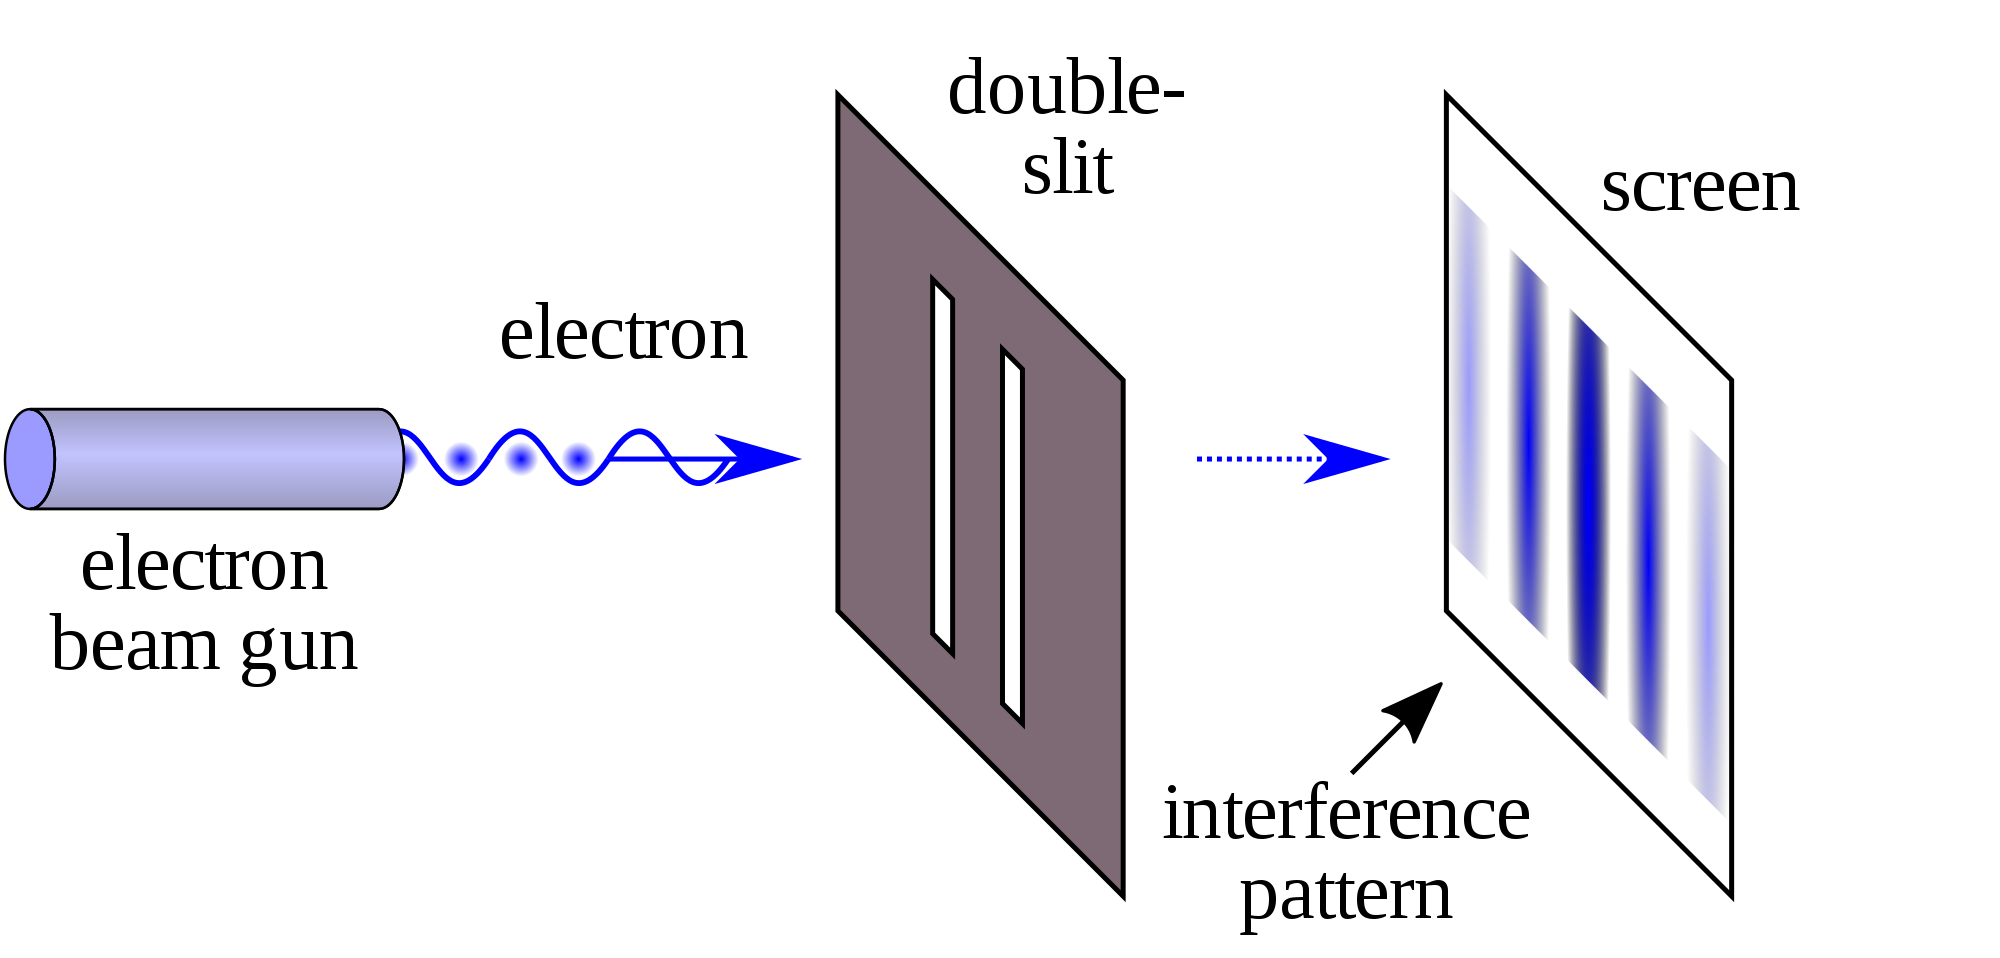
\includegraphics[width=0.6\textwidth]{figs/Etwoslitexp.png} \\
        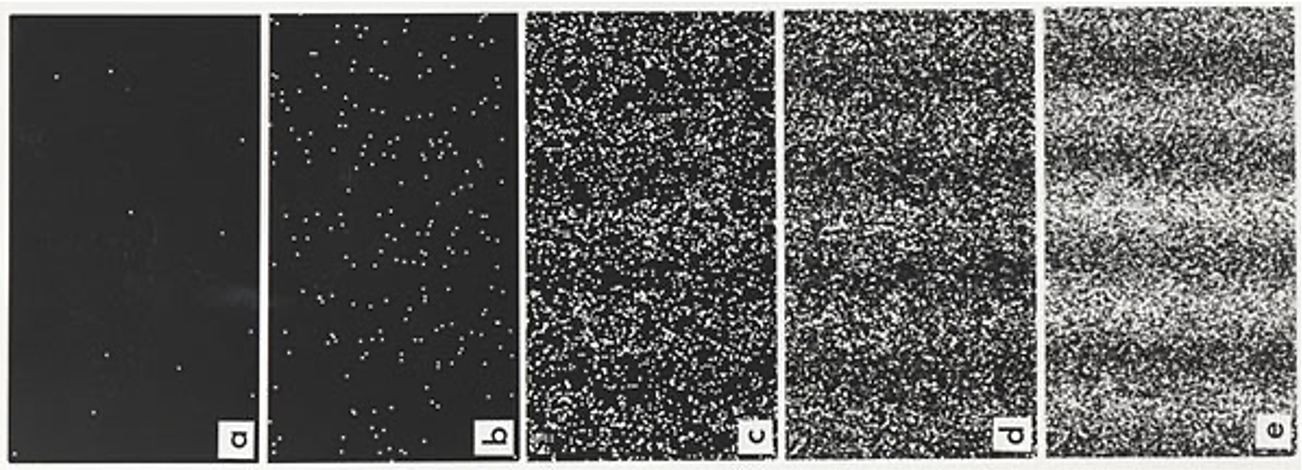
\includegraphics[width=0.6\textwidth]{figs/two-slit.png} \\
    \end{center} 
\end{frame}

\begin{frame}
    \begin{center}
        Wave-particle duality is the inherent attribute of matter \\
        ~~\\
        ~~\\
        That brings big problems in interpret the reality world! \\
    \end{center} 
\end{frame}

\begin{frame}
    \frametitle{可能结论}
    \begin{itemize}
        \item 多个波构成电子 
        \item 多个电子构成 
        \item 单个电子既是粒子又是波 
    \end{itemize}
\end{frame}

\begin{frame}
\begin{itemize}
    \item  电子与自己干涉 
    \item  电子同时过两个缝  
    \item  电子至少同时有两条路径 
    \item  牛顿力学失效! 
    \item  波动学失效! 
\end{itemize}
\end{frame}

%%%%%%%%%%%%%%%%%%%%%
\section{波函数假说}
%%%%%%%%%%%%%%%%%%%%%

\begin{frame}
    \frametitle{波函数假说}
    \begin{tcolorbox1}{Basic assumption 1/5}
    In 1924, De Broglie assumed that:\\
    The state of a system is described by a wavefunction (波函数完全描述物体的状态)
    \end{tcolorbox1}
\end{frame}

\begin{frame}
    \frametitle{构造第一个波函数}
        For the classical plane wave
        \begin{equation*}
            \begin{split}
                y(x,t)&=A e^{i(\frac{2\pi}{\lambda}x-\omega t)} \\
                    & = A e^{i\frac{2\pi}{h}(\frac{h}{\lambda}x-h\nu t)}
            \end{split} 
        \end{equation*}
        Put De Broglie relationship into the formula, we get a quantum plane wavefunction
        \begin{equation*}
            \begin{split}
                \Psi_p(x,t)&=A e^{\frac{i}{\hbar}(px-Et)}
            \end{split} 
         \end{equation*}
         It describes the state of a quantum free particle\\
         Note: Wavefunction is a complex function 
\end{frame}

\begin{frame}
    \frametitle{一般波函数}
         A general wavefunction for general particles, it should be a wave-packet of plane wavefunction
         \begin{equation*}
                \Psi(x,t)=\sum\limits_{p=0} ^{\infty} c(p)\Psi_p(x,t) = \int\limits_{p=0} ^{\infty} c(p,t) e^{\frac{i}{\hbar}px}dp
         \end{equation*}
\end{frame}


\begin{frame}
    \frametitle{德布罗意}
        \begin{columns}
            \begin{column}[t]{0.46\linewidth}
                主要成就:
                \begin{enumerate}
                    \item 物质波假说
                    \item 原子内电子的波动性
                    \item 波函数假说 
                    \item 构造第一个波函数
                \end{enumerate}
                "德布罗意已经揭开了面纱的一角"  \\
                \qquad \qquad-- 爱因斯坦 (1925) \\
                {\color{deepred} Nobel Prize in physics(1929)}
            \end{column}
            \begin{column}[t]{0.46\linewidth}
                \begin{center}
                    \includegraphics[width=0.9\textwidth]{figs/2021-12-03-18-00-05.png} \\
                \end{center} 
            \end{column}
        \end{columns}

\end{frame}

%%%%%%%%%%%%%%%%%%%%%%%%%%%%%%%%%
\section{统计诠释}
%%%%%%%%%%%%%%%%%%%%%%%%%%%%%%%%%

\begin{frame}
    \frametitle{统计诠释}
    In 1926, Born proposed statistical interpretation of wavefunction
    \begin{tcolorbox1}{Statistical interpretation}
        The magnitude of wave-function $\Psi(\vec{r},t)$ does not tell us how much of 
        the particle is at position $\vec{r}$ at time t, 
        but rather the probability (W) that the particle is at or near the position at time t. \\
        \[ d W = |\Psi(\vec{r},t)|^2 d \tau \]
    \end{tcolorbox1}
    {\color{deepred} Nobel Prize in physics(1954)}
\end{frame}

\begin{frame}
    \frametitle{解释干涉实验}
    Statistical interpretation requires wavefunction $\Psi$ to be:
    \begin{itemize}
        \item 自由电子是平面波,可以等概率出现在屏的任一位置
        \item 电子波通过双缝发生衍射和干涉,导致某些位置的振幅大,某些位置的振幅小
        \item 振幅较大的位置电子出现的概率大,形成明纹。振幅小的位置电子出现的概率小,形成暗纹
        \item 明暗干涉条纹不体现电子波的形状,体现的是电子出现概率的分布
    \end{itemize}  
\end{frame}

\begin{frame}[allowframebreaks=]
    \frametitle{数学描述}
    \begin{enumerate}
        \item Magnitude of the wave function \[|\Psi|^2 =\Psi^* \Psi \]
        \item Probability density \[\omega = |\Psi|^2 \]
        \item Probability  \[ d W = |\Psi|^2 d \tau \]
        \item Normalization \[ \int_{\Omega} |\Psi|^2 d \tau =1 \]
        \item Momentum wave-function \[ c(\vec{p},t)=\frac{1}{(2\pi\hbar)^{3/2}} \int_{0}^{\infty} \Psi(\vec{r},t) e^{\frac{-i}{\hbar} \vec{p}\cdot \vec{r} } d \tau \] 
        \item Expectation value of any function $f (x)$  \[ <f(x)>=\int_{0}^{\infty} f(x) |\Psi(x)|^2 dx \]
        \item Expectation value of observable A \[ <A>=\int_{0}^{\infty} \Psi^*(x) [A \Psi](x)| dx \]
    \end{enumerate}
\end{frame}

\begin{frame}
    \frametitle{Tips}
    \begin{itemize}
        \item $\Psi$ and $C\Psi$ describe the same state 
        \[ \frac{C\Psi(x_1)}{C\Psi(X_2)} = \frac{\Psi(x_1)}{\Psi(X_2)}\]
        \item $\Psi$ and $e^{i\varpi}\Psi$ describe the same state 
         \[ |e^{i\varpi}\Psi|^2 = e^{-i\varpi} e^{i\varpi} |\Psi|^2 = |\Psi|^2 \] 
    \end{itemize}  
\end{frame}

\begin{frame}
    \frametitle{标准化条件}
    Statistical interpretation requires wavefunction $\Psi$ to be:
    \begin{itemize}
        \item finite  function
        \item continuous function 
        \item monotropic function
        \item square integrable function (*)
    \end{itemize}
\end{frame}

\begin{frame}[allowframebreaks=]
    \frametitle{例:求归一化系数}
    \bullet 1. Normalizating the wavefunction \[\psi(x)=\sin(x), \qquad (0\le x \le \pi)\]
    \alert{Solve:} assuming the normalized wavefunction 
    \[\Psi=C\sin(x)\]
    \begin{equation*}
        \begin{split}
            \int_0 ^\pi |C\sin(x)|^2 dx &=1 \\
            C^2 \int_0 ^\pi \sin^2(x) dx &=1 \\
            C^2 \int_0 ^\pi \frac{1-\cos 2x }{2} dx &=1 \\ 
            C^2 [\frac{x}{2}-\frac{\sin 2x}{4}]_0 ^\pi &=1 \\ 
        \end{split} 
     \end{equation*}
     \[C=\sqrt{\frac{2}{\pi}}\]
     The normalized wavefunction:
     \begin{equation*}
        \Psi=C\sin(x)=\sqrt{\frac{2}{\pi}}\sin(x)
    \end{equation*}
    \bullet 2. Normalizating the plane wavefunction \[\Psi_p (x,t)=e^{\frac{i}{\hbar}(px-Et)} \] 
    \alert{Solve:} it's not a square integrable function, assuming the normalized wavefunction 
    \[\Psi=C\Psi_p (x,t)\]
    \begin{equation*}
        \begin{split}
            \int_{-\infty} ^\infty |C\Psi_p (x,t)|^2 dx &=1  \\
            C^2 \int_0 ^\infty \Psi_p (x) \Psi_{p'} (x) dx &=\delta (p-p')  \\
            C^2 \int_0 ^\infty e^{\frac{i}{\hbar}(p-p')x} =&=\delta (p-p')\\
            C^2 2\pi \hbar \delta (p-p') &=\delta(p-p') \\
            C&= \frac{1}{\sqrt{2\pi \hbar}}
        \end{split} 
     \end{equation*}
     The normalized plan wavefunction:
     \begin{equation*}
        \Psi=\frac{1}{\sqrt{2\pi \hbar}} e^{\frac{i}{\hbar}px}
    \end{equation*}  
    In general
    $$ \Psi(\vec r ,t)=\frac{1}{(2\pi \hbar)^{3/2}} e^{\frac{i}{\hbar}(\vec p\cdot \vec r -Et)} $$
    $$ \Psi(\vec r_1 ,\vec r_2, t)=\frac{1}{(2\pi \hbar)^{6/2}} e^{\frac{i}{\hbar}(\vec p_1 \cdot \vec r_1 +\vec p_2 \cdot \vec r_2 -Et)} $$
\end{frame}

\begin{frame}
    \frametitle{玻恩 (Max Born)}
        \begin{columns}
            \begin{column}[t]{0.46\linewidth}
                主要成就:
                \begin{enumerate}
                    \item 波函数的统计解释
                    \item 态叠加原理
                \end{enumerate}
                德国理论物理学家,量子力学的奠基人之一。\\
                因对波函数的统计解释,获1954年诺贝尔物理学奖.\\
                1912年受聘哥廷根大学无薪讲师,1933年因犹太血统被剥夺教职和财产,流亡英国.\\
                泡利、海森堡和黄昆都是他的学生
            \end{column}
            \begin{column}[t]{0.46\linewidth}
                \begin{center}
                    \includegraphics[width=0.9\textwidth]{figs/Born.png} \\
                \end{center} 
            \end{column}           
        \end{columns}
\end{frame}

\begin{frame}
    \frametitle{学术讨论}
    {\color{red} \Large 波函数描述的只是粒子出现的概率 ?}  
    \begin{center}
        
\includegraphics[width=0.5\textwidth]{figs/2021-12-06-11-44-50.png} \\
    \end{center} 
\end{frame}


